% !Mode:: "TeX:UTF-8"
\chapter{基于CS和FA的混合双聚类算法}
元启发式算法在双聚类领域的应用取得了很不错的效果,但元启发式算法本身的缺陷也会影响着双聚类的质量。一般来说,不同的算法有不同的使用范围,一个算法很难做到兼顾全局寻优与快速收敛。比如,布谷鸟算法具有较强的全局搜索能力,而在局部搜索却表现欠佳;萤火虫算法跟布谷鸟算法却刚好相反。全局寻优能力使得算法在寻在双聚类中能够找到更多样的结果,提高了覆盖率;局部寻优能力能够指导算法找到生物意义更加明确的双聚类结果。本文结合布谷鸟算法和萤火虫算法,提出一种混合的元启发式双聚类算法(Cuckoo Search and Firfly Algorithm hybrid Biclustering,CSFAB),并将CSFAB算法在四个基因表达数据与其他常用的双聚类算法进行了质量验证指标和生物验证指标的比较。

\section{混合双聚类算法分析}
    \subsection{编码设计}
    一般来说有两种常见的编码设计,第一种通过0和1比特串表示,第二种则是直接通过行和列的索引值来表示。对于第一种,每个解的长度是确定的,而第二种会跟随着双聚类容量的变化而变化。本文采用最为广泛使用的第一种编码方式。给定基因表达矩阵$E(X,Y)$,比特串$x_p = (g_1,\dots,g_i,\dots,g_m,s_1,\dots,s_j,\dots,s_n)$,$ p=1,\dots,N, $ 被用来表示一个双聚类或子矩阵$E(I,J)$。其中, $N,m,n$分别是种群数量,$E$的基因数目和样本数目。当$E$中第$i$个基因或第$j$个样本被选为$E(I,J)$时,$g_i=1$或$s_j=1$,否则,$g_i=0$或$s_j=0$,$1\le i \le m$ 且$1\le j \le n$。

    原始的群智能算法的解(粒子,鸟巢,萤火虫)都是多维的连续值,需要映射成对应的比特串后才能用来表示双聚类。通常的做法就是设置上限为1,下限为0,然后判断是否大于0.5,将实数值映射成比特值。如下图所示:
    \begin{figure}[htbp]
        \centering
        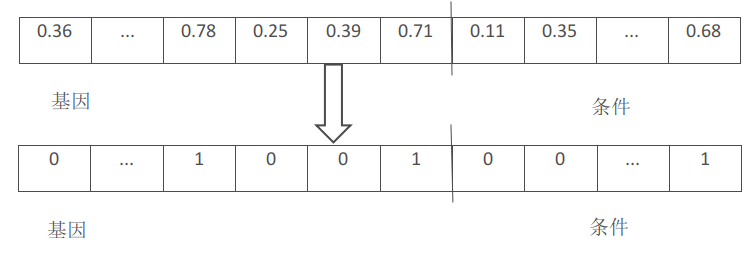
\includegraphics[width = 0.7\textwidth]{coding.png}
        \caption{将连续的解映射为双聚类}
        \label{fig:encoding}
    \end{figure}

    \subsection{适应值函数设计}\label{sec:fitness}
    优化算法需要知道优劣的评价标准,在群智能算法中一般称之为适应值。我们需要设计一个适应值函数,用来得到一个解的质量,从而在解与解之间以及算法之间进行比较。正如\ref{section:qualityEval}小节提到的,MSR是最主要也是最直观的质量评价指标,同时双聚类的体积也是衡量好坏的标准之一。一般来说,体积越大的双聚类MSR会相应的变大,而我们希望找到体积大但是MSR较小的双聚类。所以,需要在保持两者之间平衡的同时,能够引导双聚类算法找到更优的解。对于双聚类$B(I,J)$,其适应值为:
    \begin{align}
      f(B) &= MSR(B) + \frac{\lambda}{GV(B)} +\frac{\mu}{CV(B)} \\
      GV(B) & = |I| \\
      CV(B) & = |J|
    \end{align}
    其中,$GV(B)$,$CV(B)$分别是$B(I,J)$中基因和实验条件的容量。$\lambda,\mu$是针对量纲不同问题,$\lambda,\mu$越大则GV和CV对适应值的影响越大,其值视数据集的情况而定。从式中可以看出当MSR越小,基因容量和条件容量越大时,适应值越小,也就是说双聚类的质量越好。
    
    \subsection{混合方案设计}\label{sec:three}
    大致有两种策略将两个算法混合,顺序执行策略和嵌套策略。第一种策略是将一个算法的结果作为另一个算法的输入,特点是两个算法前后互不影响。例如,Nepomuceno 等将SEBI的结果输入到SSB算法中,进一步提高双聚类的质量;陈佳瑜使用量子粒子群算法的输出作为FLOC算法的输入。第二种策略是将两个算法的揉合到一起,将某一个算法作为局部功能嵌入到另一个算法中,这时两种算法前后不是独立的。例如,Bryan 等将CC算法的局部搜索功能作为SAB算法的一步,以提高双聚类的容量。基于上述二种策略,可有如下三种方案:
    \begin{enumerate}
       \item[1.] 顺序执行CS-FA:这种方案可以看作将FAB算法的随机初始化替换成CSB算法,先使用CSB算法生成双聚类,然后使用FAB算法进一步提高双聚类的质量,如算法\ref{alg:cs-fa}所示。
        \begin{algorithm}[htbp]
        \caption{CS-FA混合方案} \label{alg:cs-fa}
        % \AlgoBiCaption{这是一个简短的算法中文图题}{This is the English caption of the algorithm}
        \KwIn{$n \times m$的基因表达矩阵E,弃巢比例p,种群大小N,光吸收系数$\gamma$,最大吸引度$\beta_0$,步长因子$\alpha$,最大迭代次数Iter}
        \KwOut{一个满足条件的双聚类B}%
        P = Initialization(E, N) //初始化种群 \\
        $P_{CS}$ = CSB(P,E,p,Iter) \\
        $P_{CS-FA}$ = FAB(P,E,$\gamma$,$\beta_0$,$\alpha$,Iter) \\
        B = Best($P_{CS-FA}$) \\
        return B
        \end{algorithm}

       \item[2.] 顺序执行FA-CS:与第一种方案刚好相反,将CSB算法的随机初始化改为FAB算法,如算法\ref{alg:fa-cs}所示。
        \begin{algorithm}[htbp]
        \caption{FA-CS混合方案}\label{alg:fa-cs}
        \KwIn{$n \times m$的基因表达矩阵E,弃巢比例p,种群大小N,光吸收系数$\gamma$,最大吸引度$\beta_0$,步长因子$\alpha$,最大迭代次数Iter}
        \KwOut{一个满足条件的双聚类B}%

        P = Initialization(E, N) //初始化种群 \\
        $P_{FA}$ = FAB(P,E,$\gamma$,$\beta_0$,$\alpha$,Iter) \\
        $P_{FA-CS}$ = CSB(P,E,p,Iter) \\
        B = Best($P_{FA-CS}$) \\
        return B \\
        \end{algorithm}
       \item[3.] 嵌套执行CS-FA:该方案在每一次迭代都会执行CS操作和FA操作,并且采用竞标策略保留两次操作中最优的个体。
        \begin{algorithm}[htbp]
        \caption{CSFA混合方案}\label{alg:csfa}
        \KwIn{$n \times m$的基因表达矩阵E,弃巢比例p,种群大小N,光吸收系数$\gamma$,最大吸引度$\beta_0$,步长因子$\alpha$,最大迭代次数Iter,最大早熟次数maxEarlyStopCnt}
        \KwOut{一个满足条件的双聚类B}%
        i = 1 \\
        earlyStopCnt = 0 \\
        $B_{old}$ = INF \\
        $P_{fa}$ = Initialization(E, N) //初始化种群 \\
        \Do{(i<=Iter AND earlyStopCnt< maxEarlyStopCnt)}
        {
            $P_{cs}$, $best_{cs}$ = csIter($P_{fa}$, E, p) \\
            $P_{fa}$, $best_{fa}$ = faIter($P_{cs}$, E, $\gamma$,$\beta_0$,$\alpha$) \\
            B = Best( $best_{cs}$, $best_{fa}$) \\
            earlyStopCnt = EarlyStop(earlyStopCnt, B, $B_{old}$)
            $B_{old}$ = B \\
            i++
        }
        return B
        \end{algorithm}
    \end{enumerate}
    \subsection{停止条件}
    算法的停止条件是达到最大的迭代次数或者种群中最优双聚类的质量已经有一定的时间不再提升,后一种情况称为early stopping。通过EarlyStop函数来实现,当新的最优适应值相比较上一代的最优适应值几乎没有变化时,将earlyStopCnt加一,否则置零。
    \begin{algorithm}[htbp]
    \caption{EarlyStop函数}
    \SetAlgoLined
    \KwIn{earlyStopCnt, 新的最优适应值$f_{new}$,旧的最优适应值$f_{old}$}
    \KwOut{新的earlyStopCnt}%
        \uIf{ |$f_{new}$ - $f_{old}$| < $f_{new}/1000$}{earlyStopCnt++\;}
        \Else{earlyStopCnt = 0}
        return earlyStopCnt 
    \end{algorithm}

\section{实验环境及所用数据集}
本节主要介绍实验所用到的软硬件环境和数据,后面章节的实验所用的环境和数据与本节相同,将不再赘述。
    \subsection{实验环境}
    本文提出的CSFAB双聚类算法与其他用来比较的算法均是用Matlab语言实现,并运行在Matlab R2018b环境中。对于双聚类结果的生物验证,是用R语言的clusterProfiler包得到的。所有代码都运行在64位的Ubuntu 18.04操作系统上,CPU是intel i7-9700K,内存大小为16G。

    \subsection{实验所用数据集}
    不同的双聚类算法采取不同的搜索策略,有不同的侧重。为了全面的评估本文所提出的算法,本文选择了四个数据量各不同的数据集,如表\ref{tab:data}所示。
    \begin{table}[htbp]
    \caption{本文所用的基因表达数据集的相关信息}\label{tab:data}
    % \bicaption[table1]{}{符合研究生院绘图规范的表格}{Table$\!$}{Table in agreement of the standard from graduate school}
    \vspace{0.5em}\centering\wuhao
    \begin{tabular}{cccccc}
    \toprule[1.5pt]
    数据名缩写 & 数据全名 & 基因数量 & 条件数量 & $\lambda$& $\mu$ \\
    \midrule[1pt]
    Yeast Cell & Yeast cell cycle & 5847& 50 & 2.0E05 &  2.0E03\\
    BCLL & B-cell chronic lymphocytic leukemia& 12815& 21 & 1.0E04 & 1.0E03\\
    RatStrain & Rat multiple tissue in strain& 7751& 122 & 6.0E05 & 1.0E04\\
    PBC & Primary breast cancer& 21225& 286 & 3.0E06 & 4.0E04\\
    \bottomrule[1.5pt]
    \end{tabular}
    \end{table}
    这些基因表达数据集都是来自GEO数据库,编号分别为GDS2350,GSE2403,GSE952,GSE2034。$\lambda$和$\mu$均为经验值。本文使用Python的GEOParse包和Pandas包在基因维度上对数据进行了Min-max Normalization,缩放到[0,1]区间并乘以100。计算公式如下。
    \begin{equation}
        x^{\prime} = \frac{x - min(x)}{max(x) - min(x)} \times 100
    \end{equation}
    其中,$x$为基因表达数据的某一行,也就是该基因在所有条件下的表达水平。

\section{实验结果及分析}\label{sec:csfa_exper}
本节主要内容为三种混合方案的性能分析比较,然后在四个基因表达数据上对各双聚类算法进行测试,最后在质量验证指标和生物验证指标对各算法进行讨论分析。
    \subsection{混合方案比较}
    为了确定\ref{sec:three}节中提到的三种方案中,哪种更适合双聚类分析,本文在BCLL数据集上,使用\ref{sec:fitness}节中定义的适应值函数,分别对三种方案进行了100次实验,得到相应的双聚类。因为在算法中使用到了三个指标,为了减少偏向性,同时对相关指数RI和HV-Score共五个指标计算其平均值和标准差,如表\ref{tab:three}所示。由表\ref{tab:three}可知,前两种混合方案能够使双聚类的体积增加一些,在HV-Score 和样本个数指标上,三种策略的差别并不大,但是嵌套执行方案在MSR和RI上均有明显的优势。所以,本文抛弃了顺序执行方案,并将嵌套执行方案命名为CSFAB。

    \begin{table}[htbp]
        \caption{三种混合方案在BCLL数据集上的质量评价指标}\label{tab:three}
        \vspace{0.5em}\centering\wuhao
        \begin{tabular}{cccccc}
        \toprule[1.5pt]
         & 基因个数 & 样本个数 & MSR & RI& HV-Score \\
        \midrule[1pt]
        CS-FA  &$\bm{6093.88\pm 39.12}$& $\bm{8.03\pm 0.99$}&$296.212\pm 7.26$ & $0.019\pm 0.003$&  $0.994\pm 0.001$ \\
        FA-CS  &$6044.54\pm 51.53$& $7.54\pm 0.65$&$307.616\pm 14.17$ & $0.006\pm 0.005$&  $0.995\pm 0.001$ \\
        CSFA   &$5992.93\pm 61.52$& $8.0\pm 0.0$&\bm{$277.049\pm 2.97$} & $\bm{0.031\pm 0.003$}& \bm{$0.994\pm 0.0007$} \\
        \bottomrule[1.5pt]
        \end{tabular}
    \end{table}

    \subsection{CSFAB的质量验证指标比较分析}
    为了较公平和全面地衡量本文提出的CSFAB算法的有效性,本文选择了采用相同的编码方案和适应值函数的萤火虫算法,布谷鸟搜索算法以及粒子群算法作为对比参照算法,并分别命名为FAB,CSB,PSOB,其参数如表\ref{tab:params}所示,其中种群规模均为100。表\ref{tab:gv}和表\ref{tab:cv}分别为各算法在各数据集上的基因容量和样本容量的平均值和标准差。同时,为了评价算法的多样性,图\ref{fig:coverRate}展示了各算法在不同基因表达数据集上的覆盖率。图\ref{fig:msr}和图\ref{fig:ri}给出了各算法在在四个数据集上MSR以及RI的箱线图。
    
    从表\ref{tab:gv}可以看出,PSOB在BCLL数据集上表现最优,而CSFAB在其他三个数据集上均取得了最大的基因容量。而表\ref{tab:cv}表明,在样本容量方面,CSFAB表现平平,仅在量级最大的PBC中比另外三个算法更优,其他三个数据集均为FAB算法最优。但在BCLL中,各算法的表现相差不大。实验数据说明,在数量级比较大时,CSFAB算法更占优势。图\ref{fig:coverRate}可知,无论是在什么量级的数据中,相比其他算法,CSFAB算法总能找到更多样化的双聚类,这与殷路的研究结论保持一致。

    \begin{table}[htbp]
        \caption{CSFAB等四个算法的参数设置}\label{tab:params}
        \vspace{0.5em}\centering\wuhao
        \begin{tabular}{cc}
        \toprule[1.5pt]
        算法名 & 参数 \\
        \midrule[1pt]
        CSB & $\alpha=0.01,P_a=0.25$\\
        FAB & $\alpha=0.25,\beta_0=0.20,\gamma=1$\\
        PSOB & $w=0.6, c_1=1.80, c_2=1.00$\\
        CSFAB & $\alpha_{fa}=0.25,\alpha_{cs}=0.01,\beta_0=0.20,\gamma=1,P_a=0.25$\\
        \bottomrule[1.5pt]
        \end{tabular}
    \end{table}

    \begin{table}[htbp]
        \caption{CSFAB等四个算法的基因容量平均值与标准差}\label{tab:gv}
        \vspace{0.5em}\centering\wuhao
        \begin{tabular}{ccccc}
        \toprule[1.5pt]
         & Yeast Cell & BCLL & RatStrain & PBC \\
        \midrule[1pt]
        CSB & $2974.42\pm 41.57$& $6075.06\pm 50.18$& $3929.93\pm 47.22$& $10781.59\pm 80.67$\\
        FAB & $3034.14\pm 40.78$& $6053.57\pm 58.17$& $4126.25\pm 39.74$& $11268.66\pm 61.56$\\
        CSFAB & \bm{$3093.02\pm 37.56$}& $5992.93\pm 61.52$&\bm{$4193.04\pm 48.38$}& $\bm{11539.04\pm 82.86$}\\
        PSOB & $3030.74\pm 41.14$ & $\bm{6093.41\pm 49.89$}& $4094.83\pm 43.77$& $11052.69\pm 78.39$\\
        \bottomrule[1.5pt]
        \end{tabular}
    \end{table}

    \begin{table}[htbp]
        \caption{CSFAB等四个算法的样本容量平均值与标准差}\label{tab:cv}
        \vspace{0.5em}\centering\wuhao
        \begin{tabular}{ccccc}
        \toprule[1.5pt]
         & Yeast Cell & BCLL & RatStrain & PBC \\
        \midrule[1pt]
        CSB & $18.82\pm 0.71$& $7.86\pm 0.40$& $71.96\pm 3.96$& $202.79\pm 5.31$\\
        FAB &\bm{$23.01\pm 2.67$}&\bm{$8.03\pm 0.30$}& \bm{$80.59\pm 2.82$}& $259.41\pm 5.09$\\
        CSFAB &$18.35\pm 0.47$ & $8.0\pm 0.0$& $76.01\pm 1.79$& $\bm{267.79\pm 2.65$}\\
        PSOB &$22.66\pm 3.23$ &$7.98\pm 0.58$ & $77.08\pm 3.44$& $220.94\pm 6.76$\\
        \bottomrule[1.5pt]
        \end{tabular}
    \end{table}

    \begin{figure}[htbp]
        \centering
        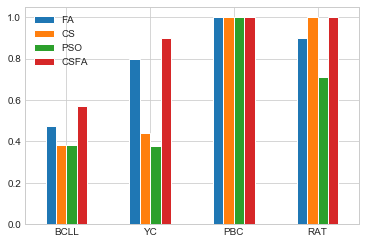
\includegraphics[width = 0.6\textwidth]{coverRate}
        \caption{CSFAB等四个算法的覆盖率}
        \label{fig:coverRate}
    \end{figure}
    从图\ref{fig:msr}可以看出,CSFAB在全部的数据集上都找得了MSR最小的双聚类,并且优势明显。一方面,这是由于适应值函数中MSR所占的比重是相对较大的,这也解释了在样本容量上,CSFAB表现并不突出;另一方面,结合Lavy飞行和萤火虫,使得算法有了更强的寻优能力。值得一提的是,CSFAB算法的四分位间距是最小的,而且其他算法出现了较多的异常点,这一现象说明了CSFAB算法要比其他三个算法更为稳定。

    \begin{figure}[htbp]
    \setlength{\subfigcapskip}{-1bp}
    \centering
    \begin{minipage}{.8\textwidth}
    \centering
    \subfigure{\label{fig:msr_bcll}}\addtocounter{subfigure}{-2}
    \subfigure{\subfigure[BCLL]{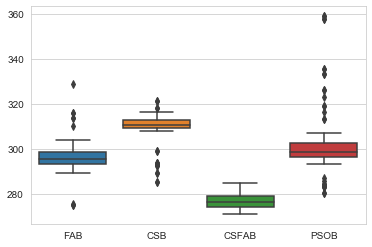
\includegraphics[width=0.4\textwidth]{msr_bcll}}}
    \hspace{.2em}
    \subfigure{\label{fig:msr_yc}}\addtocounter{subfigure}{-2}
    \subfigure{\subfigure[Yeast Cell]{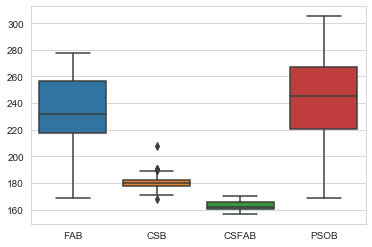
\includegraphics[width=0.4\textwidth]{msr_yc}}}
    \end{minipage}
    \centering
    \begin{minipage}{.8\textwidth}
    \centering
    \hspace{.2em}
    \subfigure{\label{fig:msr_pbc}}\addtocounter{subfigure}{-2}
    \subfigure{\subfigure[PBC]{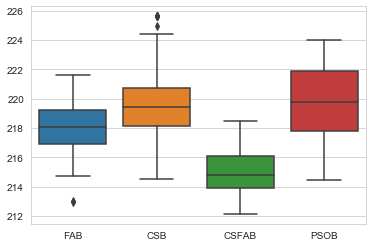
\includegraphics[width=0.4\textwidth]{msr_pbc}}}
    \hspace{.2em}
    \subfigure{\label{fig:msr_rat}}\addtocounter{subfigure}{-2}
    \subfigure{\subfigure[RatStrain]{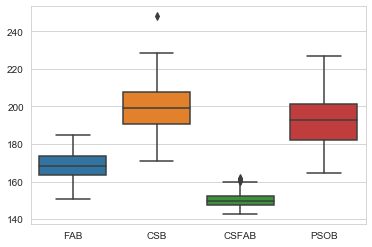
\includegraphics[width=0.4\textwidth]{msr_rat}}}
    \end{minipage}
    \vspace{0.2em}
    \caption{CSFAB等四个算法的MSR}
    \label{fig:msr}
    \end{figure}

    为了减少对MSR的倾向性,图\ref{fig:ri}展示了没有参与适应值函数的评价指标相关系数RI,值得注意的是,该指标越大则质量越好。从图中可以看出,CSFAB仅在Yeast Cell数据集紧跟在PSOB,FAB之后,另外三个数据集都取得了最优的结果。

    \begin{figure}[htbp]
    \setlength{\subfigcapskip}{-1bp}
    \centering
    \begin{minipage}{.8\textwidth}
    \centering
    \subfigure{\label{fig:ri_bcll}}\addtocounter{subfigure}{-2}
    \subfigure{\subfigure[BCLL]{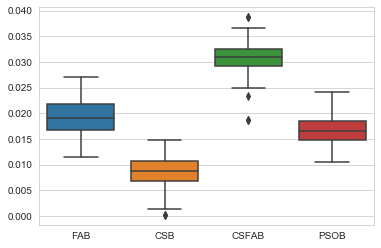
\includegraphics[width=0.4\textwidth]{ri_bcll}}}
    \hspace{.2em}
    \subfigure{\label{fig:ri_yc}}\addtocounter{subfigure}{-2}
    \subfigure{\subfigure[Yeast Cell]{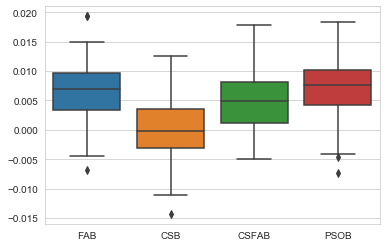
\includegraphics[width=0.4\textwidth]{ri_yc}}}
    \end{minipage}
    \centering
    \begin{minipage}{.8\textwidth}
    \centering
    \hspace{.2em}
    \subfigure{\label{fig:ri_pbc}}\addtocounter{subfigure}{-2}
    \subfigure{\subfigure[PBC]{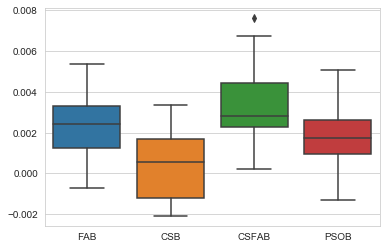
\includegraphics[width=0.4\textwidth]{ri_pbc}}}
    \hspace{.2em}
    \subfigure{\label{fig:ri_rat}}\addtocounter{subfigure}{-2}
    \subfigure{\subfigure[RatStrain]{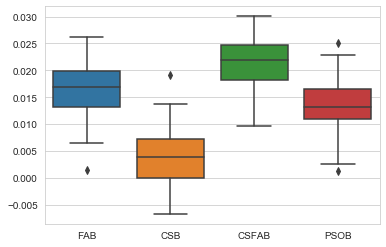
\includegraphics[width=0.4\textwidth]{ri_rat}}}
    \end{minipage}
    \vspace{0.2em}
    \caption{CSFAB等四个算法的RI}
    \label{fig:ri}
    \end{figure}

    以上分析表明,尽管CSFAB在样本容量方面没有取得足够的优势,但是在基因容量和MSR以及RI上都取得了显著的成绩。不过,对于基因表达数据的一个双聚类,最终还需要以生物质量指标来判断优劣。

    \subsection{CSFAB的生物验证指标比较分析}
    虽然CSFAB在质量评价指标上表现不俗,但是对于基因表达数据的双聚类来说,还是要找到具有生物意义的双聚类才行。因此,我们对实验中得到的双聚类进行了GO富集分析,并通过图表的方式展示。表\ref{tab:we}给出了CSFAB等四个算法的WEScore平均值与标准差。

    由表\ref{tab:we}可知,在RatStrain和PBC这两个大数据集上,CSFAB算法是最优的,而且在Yeast Cell数据集上是次优的,仅比最优的FAB低了2.5个百分点。这充分说明CSFAB算法更适合在大规模的数据上搜索相对其它算法难以搜索到的双聚类。

    \begin{table}[htbp]
        \caption{CSFAB等四个算法的WEScore平均值与标准差}\label{tab:we}
        \vspace{0.5em}\centering\wuhao
        \begin{tabular}{ccccc}
        \toprule[1.5pt]
         & Yeast Cell & BCLL & RatStrain & PBC \\
        \midrule[1pt]
        CSB & $43.59\pm 7.45$& \bm{$231.93\pm 14.10$}& $124.20\pm 44.52$& $137.90\pm 10.54$\\
        FAB &\bm{$45.76\pm 8.34$}&$230.55\pm 14.91$& $119.85\pm 41.61$& $149.24\pm 9.22$\\
        CSFAB &$44.59\pm 7.17$ & $228.71\pm 14.55$& \bm{$124.91\pm 42.06$}& $\bm{153.49\pm 12.73$}\\
        PSOB &$43.27\pm 8.03$ &$230.89\pm 14.92$ & $115.30\pm 38.60$& $143.24\pm 8.30$\\
        \bottomrule[1.5pt]
        \end{tabular}
    \end{table}
    图\ref{fig:meanP}为CSFAB等四个算法的meanPValue。与WEScore吻合的是,数据集越大,则CSFAB算法的表现越好。在规模最大的PBC数据集上,CSFAB的优势最为明显。同样在Yeast Cell数据集上是次优的,仅比最优的FAB低了0.7个百分点。

    \begin{figure}[htbp]
    \setlength{\subfigcapskip}{-1bp}
    \centering
    \begin{minipage}{.8\textwidth}
    \centering
    \subfigure{\label{fig:meanP_bcll}}\addtocounter{subfigure}{-2}
    \subfigure{\subfigure[BCLL]{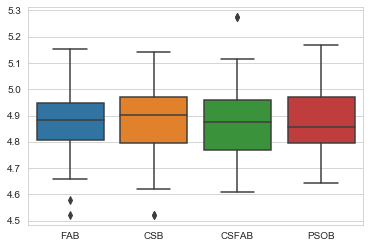
\includegraphics[width=0.4\textwidth]{meanP_bcll}}}
    \hspace{.2em}
    \subfigure{\label{fig:meanP_yc}}\addtocounter{subfigure}{-2}
    \subfigure{\subfigure[Yeast Cell]{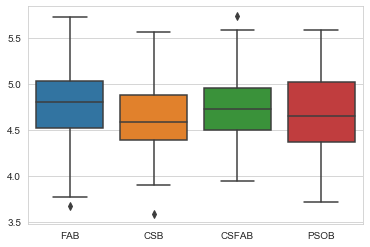
\includegraphics[width=0.4\textwidth]{meanP_yc}}}
    \end{minipage}
    \centering
    \begin{minipage}{.8\textwidth}
    \centering
    \hspace{.2em}
    \subfigure{\label{fig:meanP_pbc}}\addtocounter{subfigure}{-2}
    \subfigure{\subfigure[PBC]{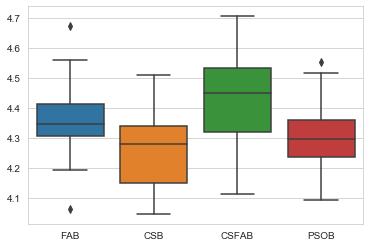
\includegraphics[width=0.4\textwidth]{meanP_pbc}}}
    \hspace{.2em}
    \subfigure{\label{fig:meanP_rat}}\addtocounter{subfigure}{-2}
    \subfigure{\subfigure[RatStrain]{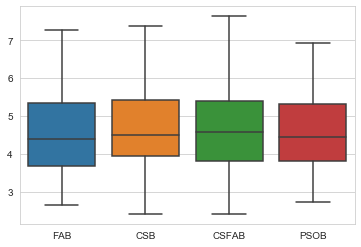
\includegraphics[width=0.4\textwidth]{meanP_rat}}}
    \end{minipage}
    \vspace{0.2em}
    \caption{CSFAB等四个算法的meanPValue}
    \label{fig:meanP}
    \end{figure}

    图\ref{fig:csfa_go_bcll}给出了CSFAB算法在BCLL数据集上某个双聚类(编号0)的部分GO富集分析结果。该双聚类包含了5923个基因和8个样本。图中其中包含了15个生物过程项,15个细胞组成项,15个分子功能项。由图\ref{fig:csfa_go_bcll}可知,该双聚类在分子功能上取得了最大的富集程度,但在其他GO项上富集的程度要比其他两种弱一些。表\ref{tab:go_term_0}给出了各类GO项中较为显著项的详细信息。从表中可以看出,该双聚类中有230个基因参与到了GO:0050839项当中,而该项的GO描述为分子功能中的细胞粘附分子结合。如果要从BCLL数据集中随机抽取5923个基因,至少包含该230个基因的概率为5.33E-23;该双聚类中有210个基因参与到了GO:0043025项中,该项为细胞组成中的神经元细胞体,其调整后的P值为6.61E-21。这些数据再一次说明了算法找到的双聚类具有明显的生物意义。
    \begin{figure}[htbp]
        \centering
        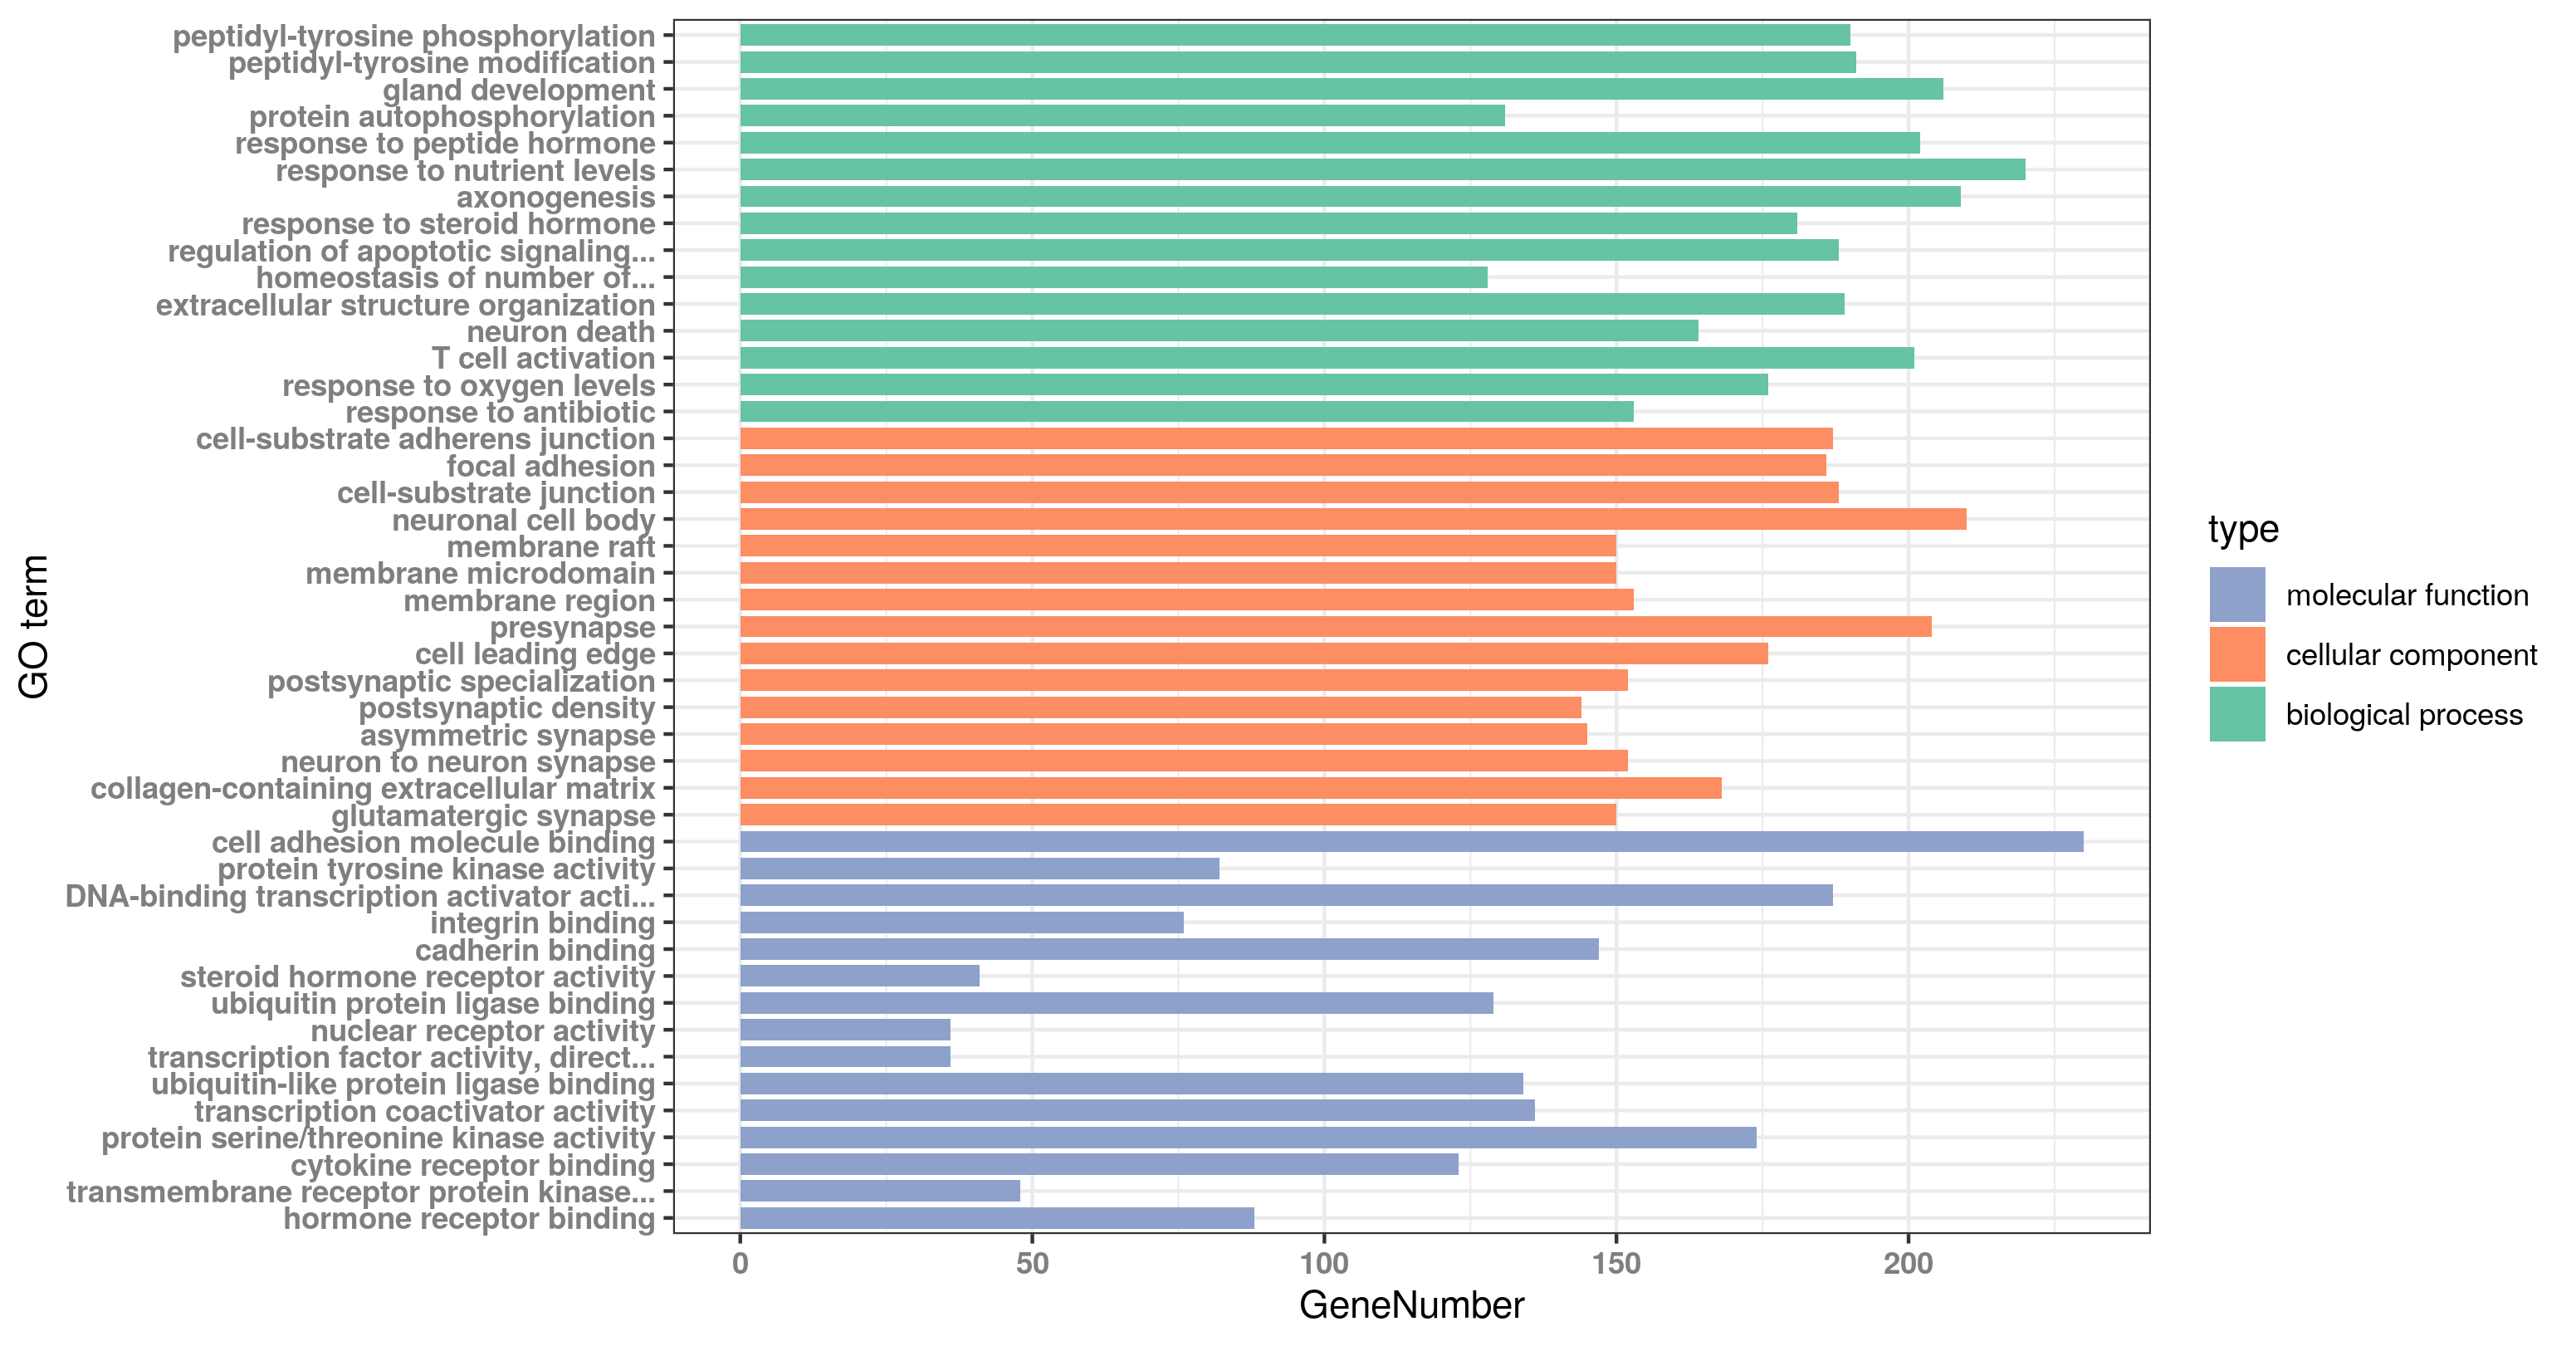
\includegraphics[width = 1\textwidth]{csfa_go_bcll_0}
        \caption{CSFAB算法得到的双聚类(编号0)主要的GO项}
        \label{fig:csfa_go_bcll}
    \end{figure}

    \begin{table}[htbp]
        \caption{双聚类(编号0)相关GO项的详细信息}\label{tab:go_term_0}
        \vspace{0.5em}\centering\wuhao
        \begin{tabular}{cccccc}
        \toprule[1.5pt]
        GOID & GO类别 &调整P值 &  基因个数 & GO描述\\
        \midrule[1pt]
        GO:0018018  &生物过程 &1.19E-29& 190& peptidyl-tyrosine phosphorylation\\
        GO:0018212  &生物过程 &1.19E-29& 191& peptidyl-tyrosine modification\\
        GO:0031667  &生物过程 &9.11E-22& 220& response to nutrient levels\\
        GO:0005924  &细胞组成 &3.44E-23& 187& cell-substrate adherens junction\\
        GO:0043025  &细胞组成 &6.61E-21& 210& neuronal cell body\\
        GO:0005925  &细胞组成 &3.44E-23& 186& focal adhesion\\
        GO:0050839  &分子功能 &5.33E-23& 230& cell adhesion molecule binding \\
        GO:0045296  &分子功能 &5.23E-13& 147& cadherin binding\\
        GO:0031625  &分子功能 &1.36E-11& 129& cell adhesion molecule binding \\
        \bottomrule[1.5pt]
        \end{tabular}
    \end{table}

\section{本章小结}
本文为了解决元启发式算法在双聚类时覆盖率不高和生物意义不明显的问题,提出了将CS算法和FA算法结合的CSFAB算法。首先提出了三种混合的方案,经实验比较后选择了嵌套执行的方案。然后,在四个数据集上对CSB,FAB和PSOB等四个算法进行了讨论分析。最后,实验证明,CSFAB算法表现稳定,不仅提高了双聚类的多样性,而且保证了其生物意义,在规模大的数据集上体现得更加明显。
